\documentclass[12pt,fleqn,a4paper,oneside]{mybook} %Final!!!

\usepackage[english]{babel}
\usepackage[utf8]{inputenc}
\usepackage[T1]{fontenc}
\usepackage{lmodern}
\pdfgentounicode=1
\usepackage{mathtools}  					
\usepackage{graphicx}
\usepackage{subfigure}
\usepackage{pdfpages}
\usepackage{enumerate}
\usepackage{etoolbox}                       %Problematic URL in reference
\apptocmd{\sloppy}{\hbadness 10000\relax}{}{}%Removes badness warnings
%This is to remove warnings resulting by otherwise OK URL's
\usepackage[hyphens]{url}
\usepackage{notes}
\usepackage{indentfirst}
\usepackage{makecell}
\renewcommand\theadfont{\bfseries\sffamily}
\usepackage{upgreek}
\usepackage{multicol}
\usepackage{eurosym}
%This custom command defines how the literal menus look like.
\newcommand{\gui}[1]{{\emph{#1}}} %Gui commands, icon names, buttons
% All code, functions, variables are typed like this
\newcommand{\code}[1]{{\lstinline[columns=fixed]{#1}}}

\newcommand{\angl}[1]{{\footnote{\emph{angl.}\ {#1}}}} %Shorthand english equivalent

\usepackage[inner=3.5cm,outer=2cm,top=25mm,bottom=25mm,paperwidth=210mm,paperheight=297mm,includehead]{geometry}

\usepackage{titlesec}
\titleformat{\chapter}[hang]{\normalfont\huge\bfseries}{\thechapter}{1em}{}


\DeclarePairedDelimiter{\diagpars}{(}{)}
\newcommand{\diag}{\operatorname{diag}\diagpars}

\let\oldhat\hat
\renewcommand{\vec}[1]{\boldsymbol{\mathbf{#1}}}

\usepackage{amsthm}
\usepackage{etoolbox}% http://ctan.org/pkg/etoolbo
\theoremstyle{definition}
\newtheorem{exmp}{Pr\'{i}klad}[chapter]
\AtEndEnvironment{exmp}{\null\hfill\qedsymbol}

\usepackage{listings,color} 			    %To list Matlab code

\usepackage{xcolor}

\definecolor{Myblack}{RGB}{48, 55, 54}
\definecolor{Mybrown}{RGB}{15, 153, 117}
\definecolor{Mygreen}{RGB}{160, 82, 131}
\definecolor{Myyellow}{RGB}{208, 170, 91}
\definecolor{Myblue}{RGB}{4, 118, 249}

\lstset{language=C++,
	basicstyle=\ttfamily,
	keywordstyle=\color{Myblue}\ttfamily,
	stringstyle=\color{Myyellow}\ttfamily,
	commentstyle=\color{Mygreen}\ttfamily,
	numbers=none,
	breaklines=true,
	showspaces=false,
	showstringspaces=false
	backgroundcolor=\color{white}, % set backgroundcolor
	basicstyle=\footnotesize,% basic font setting
	morecomment=[l][\color{Mybrown}]{\#}
}
\renewcommand\lstlistingname{Code}
\renewcommand\lstlistlistingname{Code listing}

\pagestyle{empty}

\begin{document}
	%%%%%%% beginning %%%%%%%%
	
\includepdf[pages={1}]{titlePage.pdf}
	\frontmatter
	\tableofcontents
	\thispagestyle{empty}
	\cleardoublepage
	\setcounter{page}{1}
	% \phantomsection
	\addcontentsline{toc}{chapter}{\listfigurename}
	\listoffigures
	\cleardoublepage
	% \phantomsection
	\addcontentsline{toc}{chapter}{\lstlistlistingname}
	\lstlistoflistings
	\newpage
	%%%%%% Jednotlive kapitoly %%%%%%%%%
	\pagestyle{plain}
	\pagenumbering{arabic}
	\setcounter{page}{1}
	
	\mainmatter
	\chapter*{Introduction}
\label{Introduction}
\addcontentsline{toc}{chapter}{Introduction}

In the field of control systems, the inverted pendulum stands as a classic and challenging problem, serving as a benchmark for testing the capabilities of control algorithms \cite{HAMZA2019347}. This project delves into the domain of inverted pendulum dynamics, focusing on the design, simulation, and implementation of control algorithms to stabilize and control the system dynamics.

The inverted pendulum, with its inherent instability, demands precise control strategies to maintain equilibrium. Our objective is to investigate and implement four known plus one new control methodologies that not only stabilize the pendulum in its upright position but also exhibit robust performance in the face of disturbances and uncertainties.

The report encompasses the theoretical foundations of control systems for inverted pendulum. Subsequently, it delves into the specific challenges posed by inverted pendulum dynamics and the various control strategies that have been proposed in the literature such as Jezierski, Mozaryn and Suski \cite{LQRvsMPC}, book "The Inverted Pendulum in Control Theory and Robotics" \cite{bookInverted} or the book "Advanced Control of Wheeled Inverted Pendulum Systems" \cite{controlInverted}.

\begin{figure}[!tbh]
	\hfill
	\subfigure[Rotational inverted pendulum from the company quanser \cite{Quanser_2023}.]{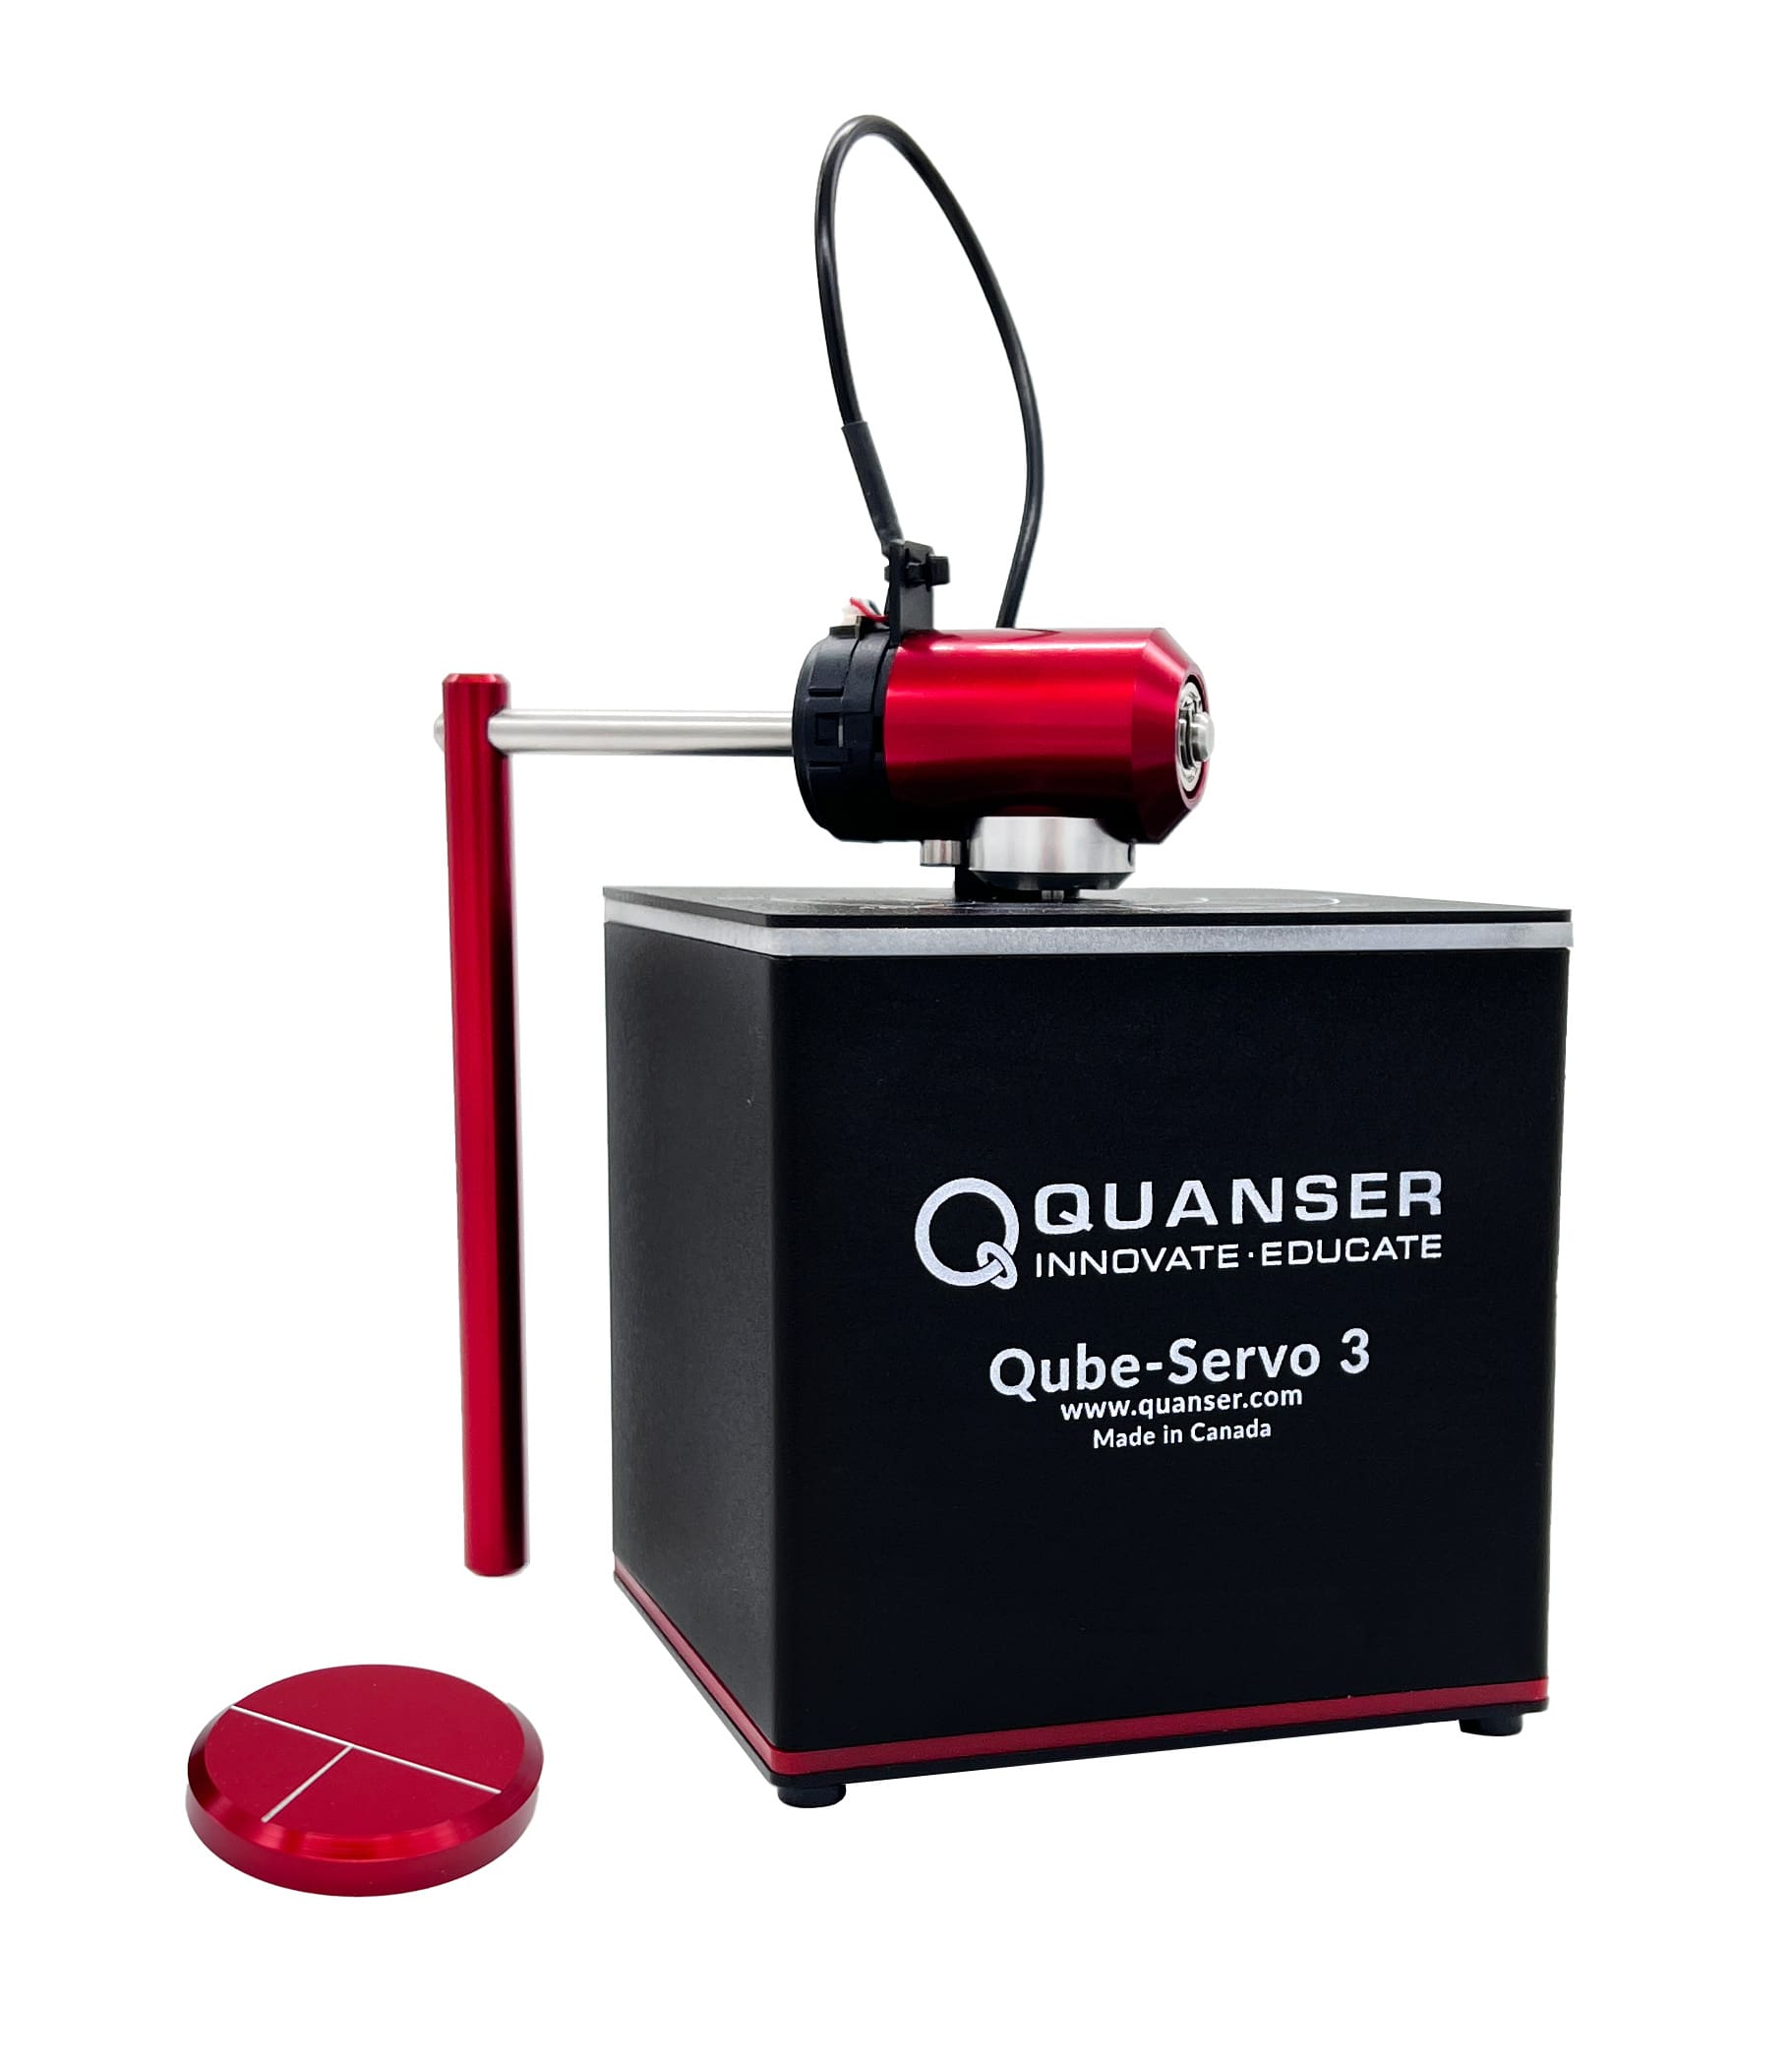
\includegraphics[width=6cm]{obr/rotationalPendulum.jpg}}
	\hfill
	\subfigure[Linear inverted pendulum from the company quanser \cite{Quanser_2023a}.]{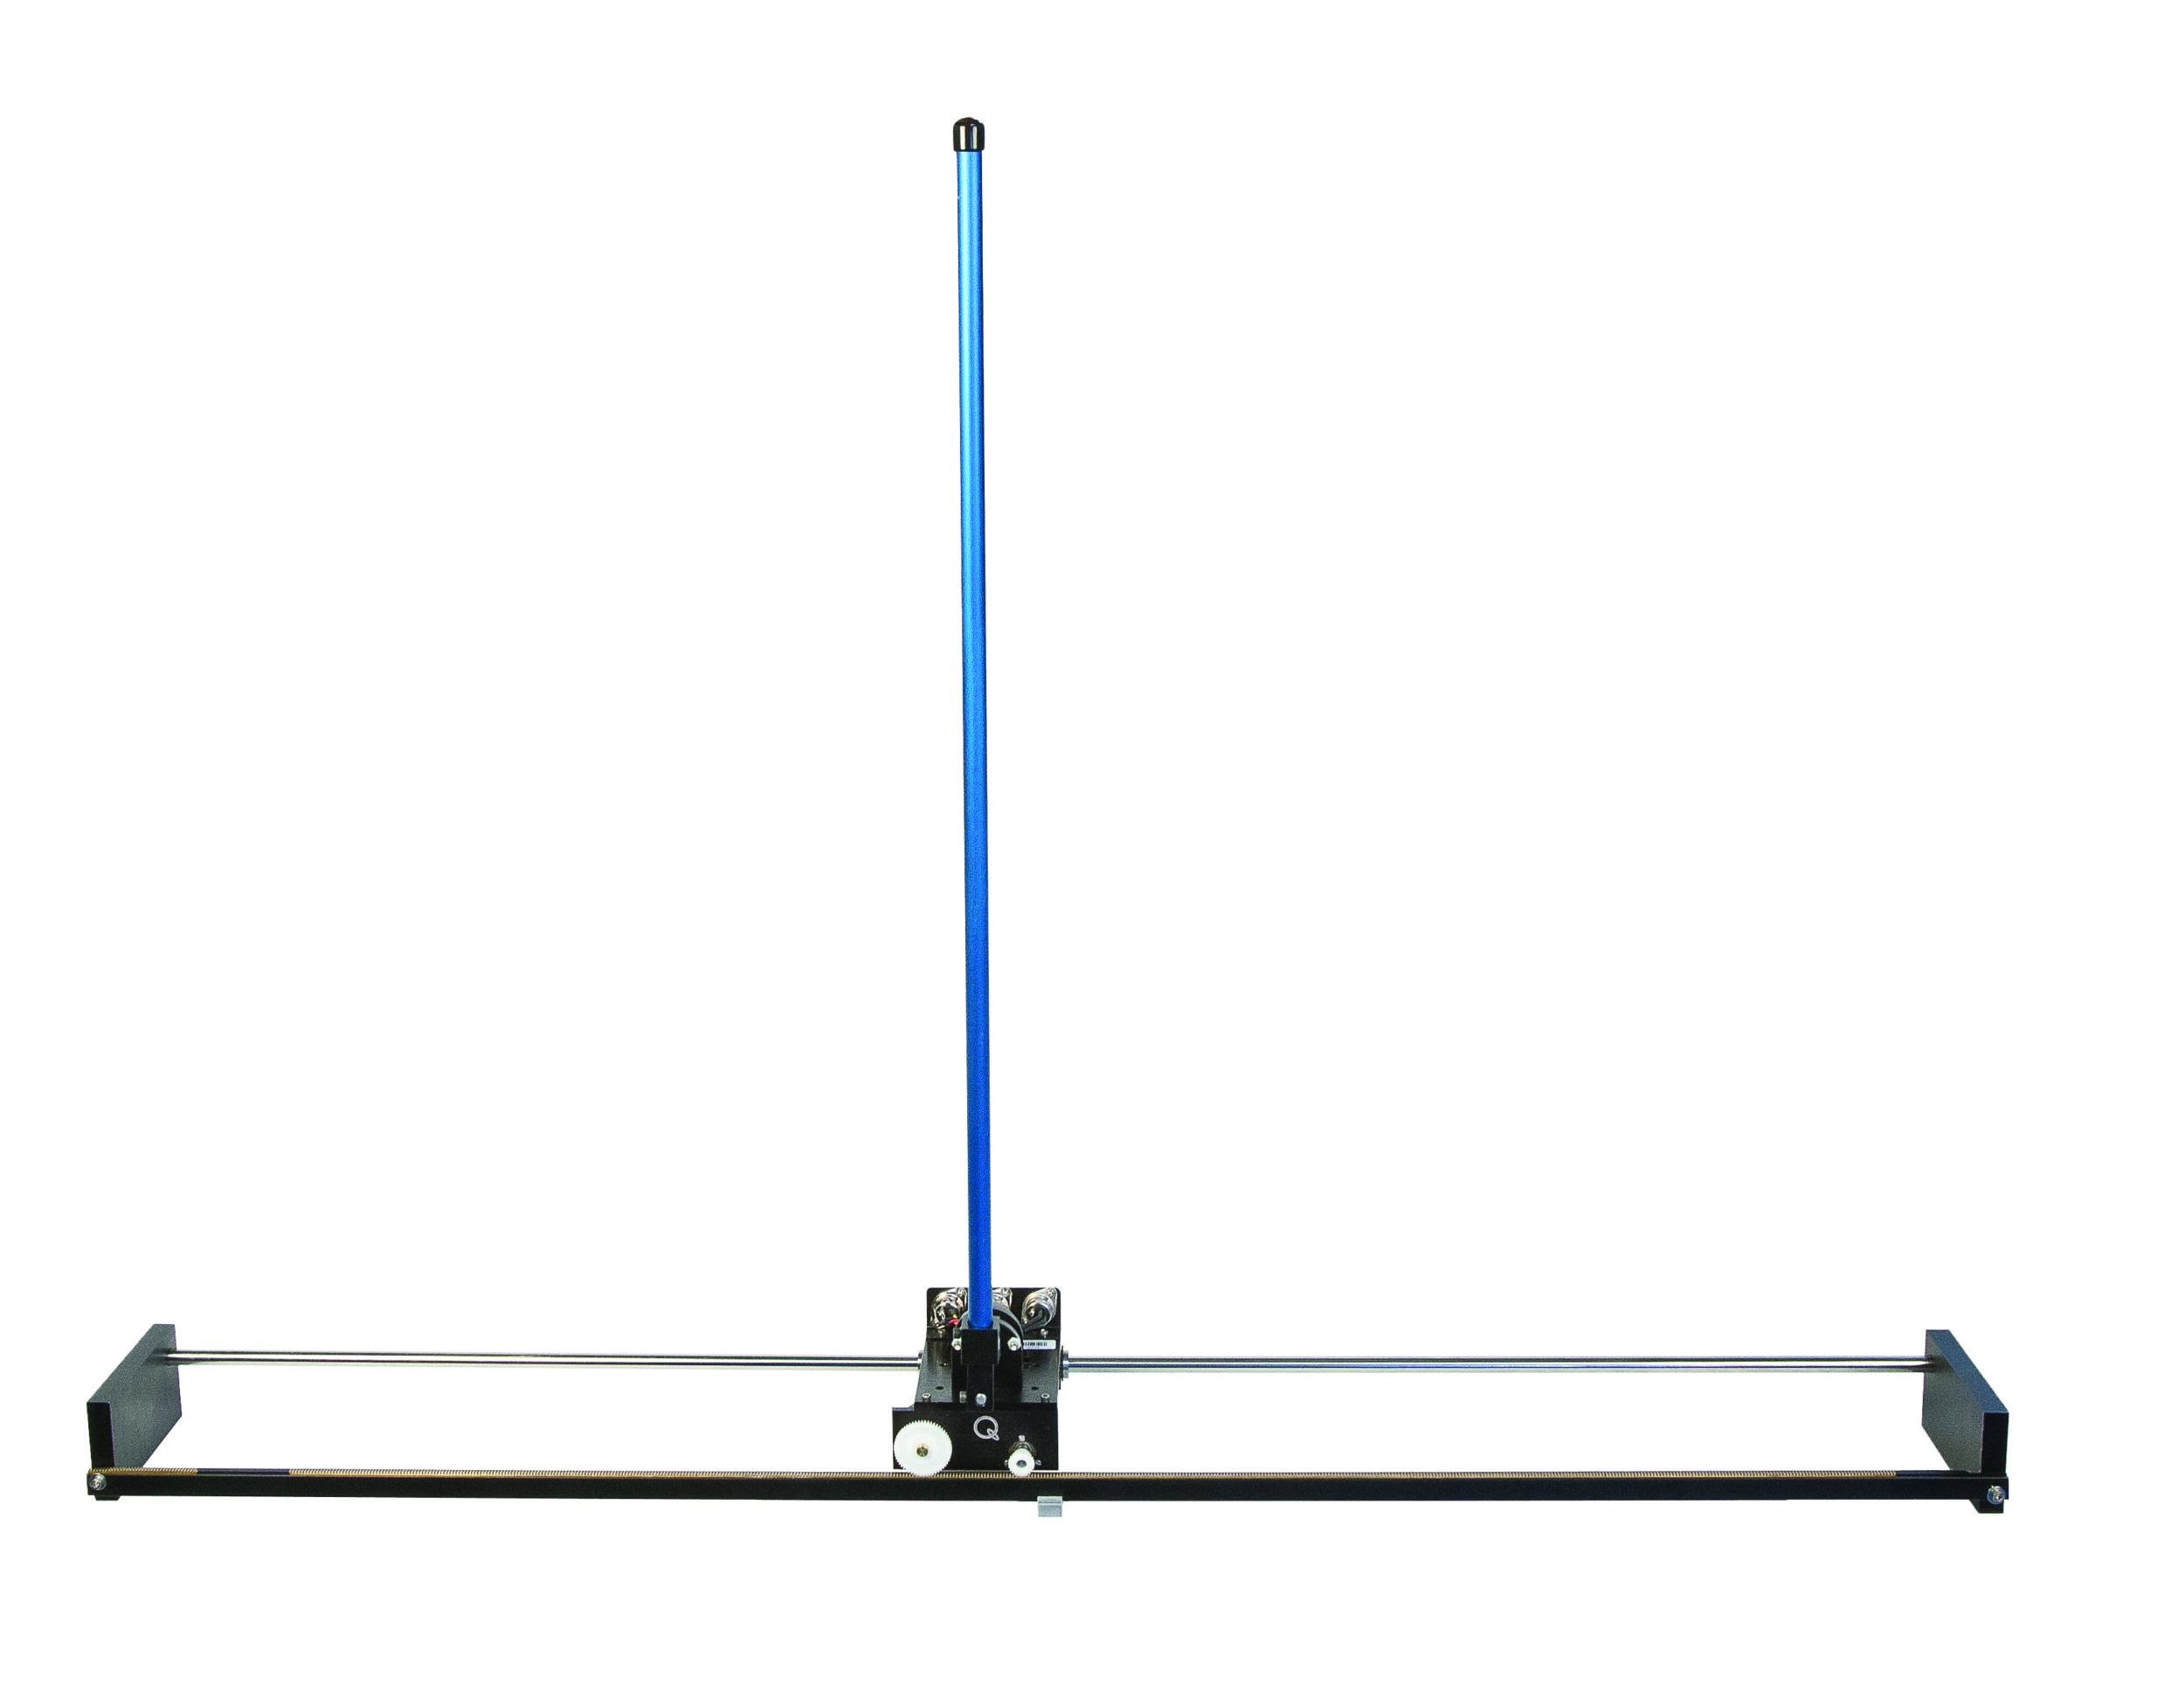
\includegraphics[width=8cm]{obr/linearPendulum.jpg}}
	\hfill
	\caption{Configurations of inverted pendulum.}\label{RotAndLin}
\end{figure}

Within the domain of inverted pendulum systems, there are two main types of configurations. It is rotational Fig. \ref{RotAndLin}.a and linear configuration Fig. \ref{RotAndLin}.b. In the case of a rotational inverted pendulum, the focus lies on managing the rotational motion of an object around a fixed pivot point. A classic example is a rigid rod attached to a pivot, and other fixed rod attached to the end of it, where the objective is to stabilize the system in an inverted position despite its inherent instability.

On the other hand, a linear inverted pendulum involves translational or linear motion along a vertical axis. This configuration is often represented by a cart on a track, with a pendulum attached to the cart. The task is to control the linear motion of the cart to maintain equilibrium with the pendulum inverted. The setup we are using for simulation and real world implementation is the linear model of inverted pendulum. 

Our focus extends beyond theoretical considerations, as the project involves practical implementation on a physical inverted pendulum setup which is located at the chair of Automation and Control of RPTU. This particular setup can be seen on the picture \ref{PICTURE_PENDULUM}. The hardware experimentation provides valuable insights into the real-world applicability of the developed algorithms, offering a bridge between theory and application.

\begin{figure}[!tbh]
	\centering
	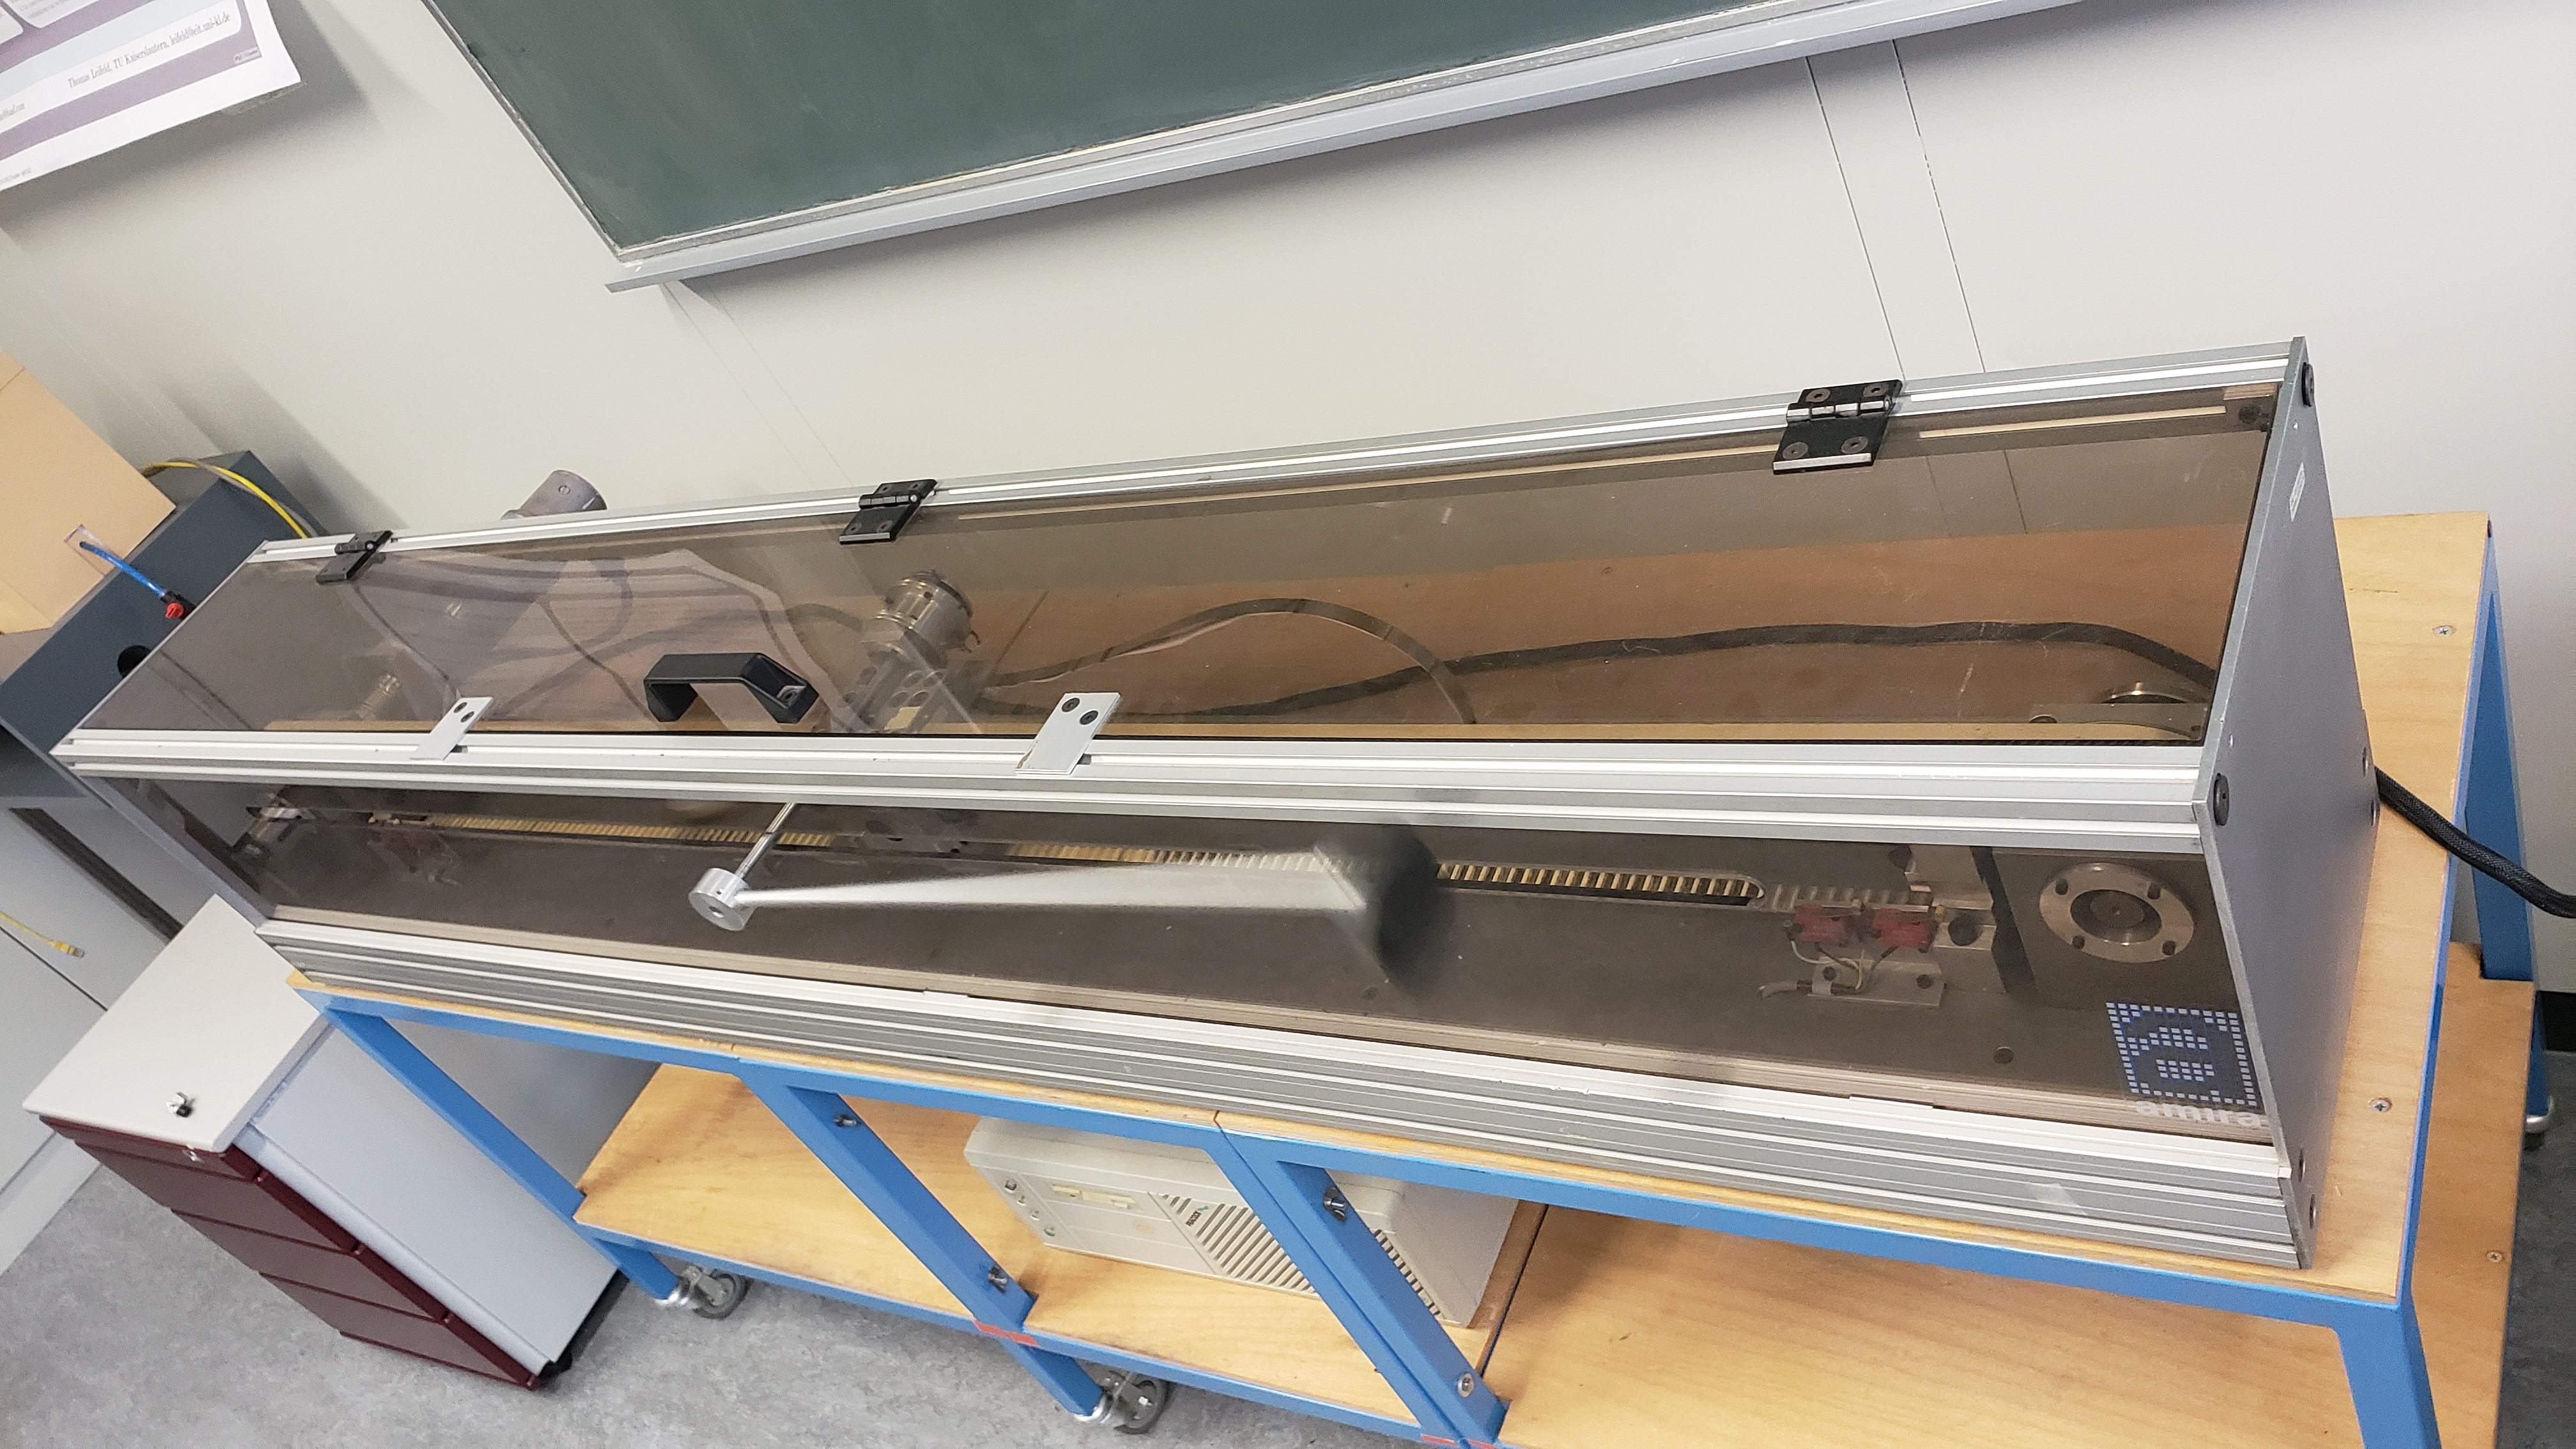
\includegraphics[width=140mm]{obr/pendulumInverted.jpg}
	\caption{Inverted pendulum setup on which implementation of designed controllers was done.}\label{PICTURE_PENDULUM}
\end{figure}

This project aims to contribute to the field of control systems by presenting a comprehensive exploration of control algorithms for inverted pendulum systems. Through rigorous analysis and experimentation, this report endeavors to showcase the effectiveness and adaptability of the implemented control algorithms, opening avenues for further advancements in the control of dynamic systems.

	\chapter{Hardware}
\section{Inverted pendulum}
\section{Controller}

\chapter{Software}


\chapter{Controllers}
\section{Linear quadratic regulator (LQR)}
\subsection{Theory}
The Linear Quadratic Regulator (LQR) has been presented by Rudolf E. Kalmanin in 1960 \cite{lqrLecture}. This optimal control algorithm is used for stabilizing linear dynamic systems by determining a control input that minimizes a quadratic cost function. LQR is an unified systematic control method for multiple-input multiple-output (MIMO) systems \cite{lqrLecture}. It is a very popular control algorithm because of its inherent robustness, where the gain and phase margin are guaranteed \cite{1102565}. 

Central to the LQR framework is the concept of linear system dynamics. LQR is tailored for linear time-invariant systems, typically characterized by matrices A, B, C, and D, encapsulating the system's behavior \cite{wikiLQR}.

At its core, LQR revolves around the minimization of a quadratic cost function over a specified time horizon. LQR reduces the amount of labor that needs to be put into the design of the controller, although the formulation of the cost function plays a crucial role in the controller performance.

The solution to the LQR problem involves online and offline calculations that can be separated to three distinct parts \cite{lqrLecture}:
\textbf{
\begin{enumerate}
	\item Solving the Riccati differential equation \footnote{Riccati differential equation is a type of first-order ordinary differential equation that has a quadratic term in one of its variables} 
	\item Computation of the feedback matrix K*\(t\)
	\item Evaluation of the feedback control law
\end{enumerate}
} 

Linear quadratic control problem can be formulated as Eq. \ref{eq1}
\begin{equation}\label{eq1}
\underset{x(t),u(t).t_e}{min}J(x(t),u(t),t_e)\: with \: J=\frac{1}{2}x(t_e)^TSx(t_e)+\frac{1}{2}\int_{0}^{t_e}x(t)^TQ(t)x(t)+u(t)^TR(t)u(t)dt
\end{equation}
where $x(t_e)$ is the end state vector, $Q(t)$ is the state weighting matrix, $R(t)$ is the input weighting matrix and $S$ is the end weighting matrix. Weighting matrices $Q,R$ and $S$ are design parameters and with the help of them, we can change the behavior of the controller. The optimal feedback control law is give by Eq. \ref{eq2} \cite{lqrLecture}

\begin{equation}\label{eq2}
u^*(t)=K^*(t)x(t)
\end{equation}

where $K^*$ is the feedback matrix. given by Eq. \ref{eq3} \cite{lqrLecture}
\begin{equation}\label{eq3}
K^*(t)=R(t)^{-1}B(t)^TP(t)
\end{equation}

\subsection{Simulation}
In the context of simulation using MATLAB for control system design, the provided code, obtained from the lab coordinator, incorporates the design of a Linear Quadratic Regulator (LQR) controller used for the control of nonlinear inverted pendulum. The primary objective is to evaluate the functionality of the code under different conditions. To assess the system's robustness and performance, disturbances have been introduced. Additionally, the LQR controller's parameters have been fine-tuned for optimal performance.

The simulation relies on MATLAB's dlqr command Eq. \ref{eq3andHalf}, where "dlqr" stands for "Linear-quadratic (LQ) state-feedback regulator" specifically designed for discrete-time state-space systems. This MATLAB command is instrumental in computing the state-feedback gain matrix for an LQR controller, considering both state and input weighting matrices. The resulting gain matrix is then utilized in the feedback control law to regulate the system and optimize its performance. 
\begin{equation}\label{eq3andHalf}
[K,P]=dlqr(A,B,Q,R)
\end{equation}
Where $K$ is the feedback matrix and $P$ infinite horizon solution of the associated discrete-time Riccati equation, where $P$ is in the form of Eq. \ref{eq4}

\begin{equation}\label{eq4}
A^TSA-S-(A^TSB+N)(B^TSB+R)^{-1}(B^TSA+N^T)+Q=0
\end{equation}

\begin{figure}[!tbh]
	\centering
	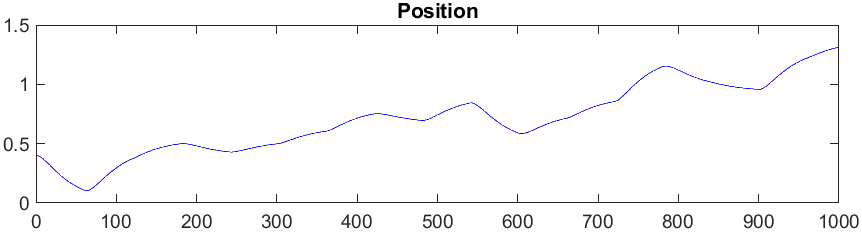
\includegraphics[width=130mm]{obr/position.png}
	\caption{Position of the pendulum $($LQR simulation$)$.}\label{lqrpos}
\end{figure}

\newpage
\subsection*{Simulation outputs}
Following the MATLAB simulation, the obtained results reveal distinctive patterns Fig. \ref{lqrpos}, \ref{lqrang}, \ref{lqrTorq}. Notably, each spike observed across all plots corresponds to the introduced disturbance. These disturbances were deliberately added to assess the robustness of the controller under varying conditions.

Figure \ref{lqrpos} shows the changing position of the pendulum carriage. Figure \ref{lqrang} shows the angle of the pendulum in radians and Fig. \ref{lqrTorq} shows the force i.e. torque applied, to move the pendulum. The full code can be found in appendix on the page \pageref{lqrSim.m}.



\begin{figure}[!tbh]
	\centering
	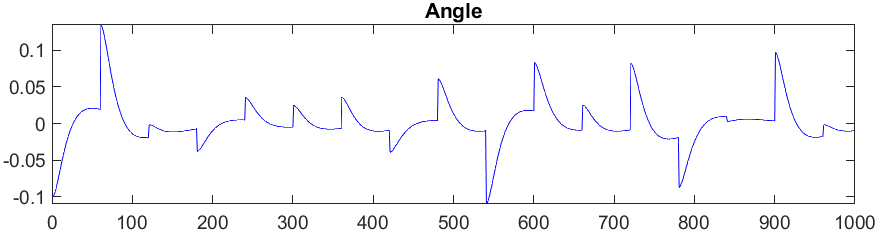
\includegraphics[width=130mm]{obr/lqrangle.png}
	\caption{Angle of the pendulum $($LQR simulation$)$.}\label{lqrang}
\end{figure}

\begin{figure}[!tbh]
	\centering
	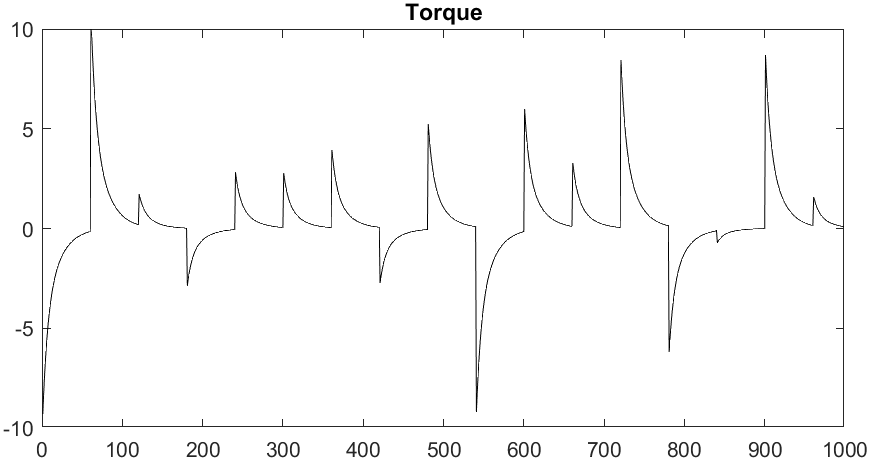
\includegraphics[width=130mm]{obr/torquelqr.png}
	\caption{Torque of the pendulum $($LQR simulation$)$.}\label{lqrTorq}
\end{figure}

Examining the plots, it becomes apparent that the angle of the pendulum Fig. \ref{lqrang} achieves stabilization in the unstable upright position within a maximum of 20 samples, depending on the level of disturbance introduced. However, it's important to note that the position of the pendulum Fig. \ref{lqrpos} does not attain stability; instead, it undergoes movement away from its initial 0 position $($when trying to control the pendulum angle$)$.

\subsection{Implementation}

\newpage
\section{Model predictive control (MPC)}
\subsection{Theory}
Model Predictive Control (MPC) represents an optimal control methodology where the computed control actions are designed to minimize a cost function for a constrained dynamical system over a finite, receding horizon. Its primary advantage over LQR control lies in its superior performance when the process encounters limitations \cite{zaklPredRiad}. However, it is acknowledged that MPC require a steeper learning curve and a more intricate implementation process. Often compared to playing chess, MPC depends on a deep understanding of the plant model and subsequent predictions of its behavior, recalculating the best possible output at each step \cite{zaklPredRiad}\cite{mpcLecture}.

In the MPC framework, the controller, at each time step, receives or estimates the current state of the plant. Based on this information, it computes a sequence of control actions that minimizes the cost over the specified horizon $($horizon can be sometimes infinite$)$ \cite{matlabMPC}\cite{zaklPredRiad}. This involves solving a constrained optimization problem, heavily relying on an internal plant model and dependent on the current system state. The controller then applies the first computed control action to the plant, disregarding the subsequent ones \cite{matlabMPC}. This iterative process repeats in each subsequent time step.

In practical applications, despite the finite horizon, MPC inherits several beneficial characteristics from traditional optimal control methodologies. It naturally accommodates multi-input multi-output (MIMO) plants, time delays, and possesses inherent robustness against model errors \cite{mpcLecture}. Furthermore, nominal stability can be assured by incorporating specific constraints. Overall, while MPC demands a more intricate knowledge of the system and involves a complex implementation, it gives big advantages in handling constraints and offering superior performance \cite{zaklPredRiad}.

In a mathematical way we can express MPC problem as: finding the best control sequence over a future horizon of N steps Eq. \ref{mpc1}
\begin{equation}\label{mpc1}
\underset{u_o,...,u_{N-1}}{min}\sum_{k=0}^{N-1}\left \| y_k-r(t) \right \|_{2}^{2}+\rho \left \| u_k-u_r(t) \right \|_{2}^{2}
\end{equation}
\begin{align}
s.t.	x_{k+1}&=f(x_k,u_k) \label{mpc2}\\ 
	y_k &=g(x_k) \nonumber
\end{align}
\begin{align}
	u_{min}\leq u_k\leq u_{max} \label{mpc3}\\
	y_{min}\leq y_k\leq y_{max} \nonumber
\end{align}
\begin{equation}\label{mpc4}
	x_o=x(t)
\end{equation}

Where Eq. \ref{mpc2} stands as the prediction model, Eq. \ref{mpc3} as constraints and Eq. \ref{mpc4} as state feedback \cite{mpcLecture}. 

\subsection{Simulation}

HOW WAS THE SIMULATION DONE\\

Following the MATLAB simulation, the obtained results reveal distinctive patterns Fig. \ref{mpcPos}, \ref{mpcAng}, \ref{mpcTor}. Notably, each spike observed across all plots corresponds to the introduced disturbance. These disturbances were deliberately added to assess the robustness of the controller under varying conditions.

Figure \ref{mpcPos} shows the changing position of the pendulum carriage. Figure \ref{mpcAng} shows the angle of the pendulum in radians and Fig. \ref{lqrTorq} shows the force i.e. torque applied, to move the pendulum. The full code can be found in appendix on the page \pageref{mpcSim.m}.

\begin{figure}[!tbh]
	\centering
	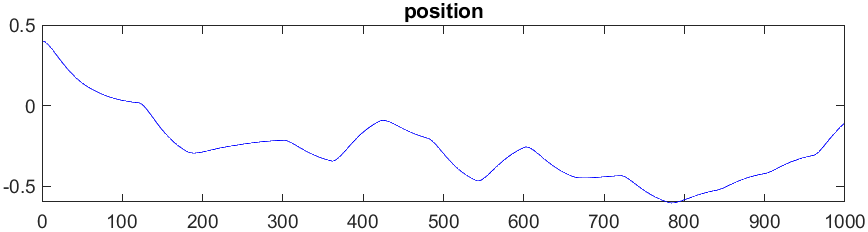
\includegraphics[width=150mm]{obr/mpcPos.png}
	\caption{Position of the pendulum $($MPC simulation$)$.}\label{mpcPos}
\end{figure}

\begin{figure}[!tbh]
	\centering
	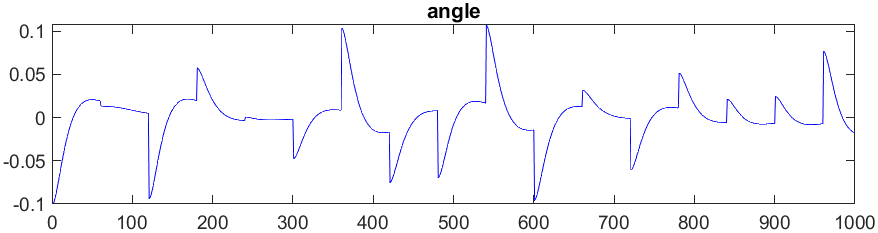
\includegraphics[width=150mm]{obr/mpcAng.png}
	\caption{Angle of the pendulum $($MPC simulation$)$.}\label{mpcAng}
\end{figure}

\begin{figure}[!tbh]
	\centering
	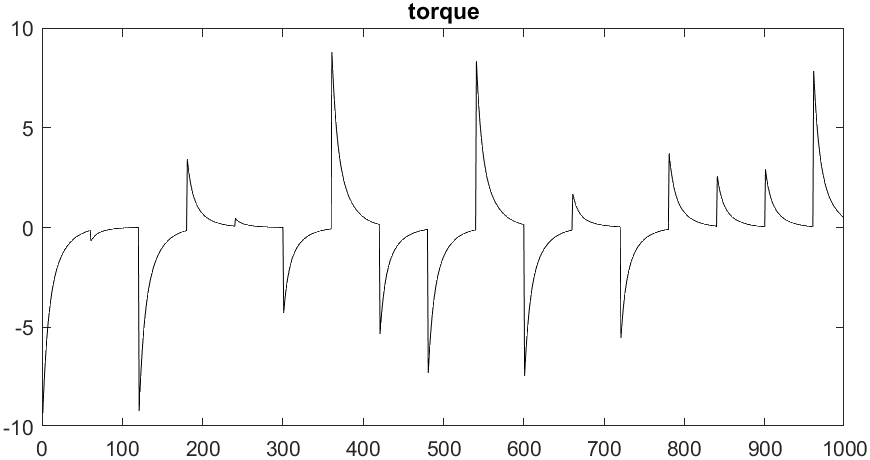
\includegraphics[width=150mm]{obr/mpcTor.png}
	\caption{Torque of the pendulum $($MPC simulation$)$.}\label{mpcTor}
\end{figure}

Examining the plots, it becomes apparent that the angle of the pendulum Fig. \ref{mpcAng} achieves stabilization in the unstable upright position within a maximum of 20 samples, depending on the level of disturbance introduced. However, it's important to note that the position of the pendulum Fig. \ref{mpcPos} does not attain stability; instead, it undergoes movement away from its initial 0 position $($when trying to control the pendulum angle$)$.

\subsection{Implementation}

\newpage
\section{Sliding mode control (SMC)}
\subsection{Theory}

Sliding mode control (SMC) is a nonlinear control methodology known for its impressive attributes such as precision, resilience, and straightforward tuning and application. It is applicable to both Single-Input Single-Output (SISO) and Multiple-Input Multiple-Output (MIMO) systems \cite{slidingLecture}\cite{Decarlo2008AQI}. The SMC consists of a two-part controller design. In the initial phase, an N-dimensional sliding surface must be designed where, by definition, the error asymptotically approaches zero. The subsequent phase is concerned with the selection of a control law, that will make the system states be attracted to the sliding surface.

The state-feedback control law is not a continuous function of time, rather, it can transition from one continuous structure to another based on the current position in the state space. The movement of the system as it glides along the boundaries of the control structures is referred to as a sliding mode, and the geometric locus comprising these boundaries is called the sliding surface \cite{wikiSMC}. SMC exhibits robustness against model uncertainties and disturbances. However, a significant drawback is the occurrence of chattering effects around the surface, which arises as a result of the switching of the control law. This is a common phenomenon in sliding mode control and is highly undesirable in practical applications due to increased control activity and the potential excitation of unmodeled high-frequency dynamics. Nevertheless, these issues can be mitigated or even avoided through the application of appropriate strategies \cite{slidingLecture}.

\subsection{Simulation}

The initial stage in simulating the sliding mode controller in MATLAB involved the creation of the sliding surface Eq. \ref{smcL1}. Afterwards, the calculation of the output estimate $\tau$ Eq. \ref{smcL5} needs to be done. 

\begin{align}
s &= (\frac{d}{dt}+e)\tilde{\alpha }+(\frac{d}{dt}+\beta )\tilde{\rho}=\dot{\tilde{\alpha }}+e\tilde{\alpha }+\dot{\tilde{\rho }}+\beta \tilde{\rho }=-\dot{\alpha }-e\alpha -\dot{\rho }-\beta \rho =0 \label{smcL1}\\
\dot{s} &=-\dot{\omega }-e\omega -\dot{v}-\beta v=0 \label{smcL2}\\
\dot{s} &=-\frac{}{}\varphi -\frac{}{}\alpha +\frac{}{}\tau +(\frac{}{}-e)\omega +\frac{}{}v-\frac{}{}\tau -\beta v \label{smcL3}\\
\dot{s} &= \label{smcL4}\\
\hat{\tau } &=\frac{j_a(m_\omega +m_e)}{m_el_{sp}-j_a}\left ( \frac{}{}+\frac{}{}-(\frac{}{}-e) -(\frac{}{}-\beta )v\right ) \label{smcL5}\\
\hat{\tau } &= \nonumber\\
\hat{\tau } &=12,335239v+68,877358\alpha -3,492138(0,125-e)\omega -3,492138(1,7568-\beta )v \nonumber
\end{align}

where $q_2$ stands for the pendulum angle, $\dot{q_2}$ is the angular velocity of the pendulum, $q_1$ is position of the base of the pendulum and $\dot{q_1}$ is the linear velocity of the base of the pendulum.

Following the MATLAB simulation, the obtained results reveal distinctive patterns Fig. \ref{posSmc}, \ref{angSmc}, \ref{torSmc}. Notably, each spike observed across all plots corresponds to the introduced disturbance. These disturbances were deliberately added to assess the robustness of the controller under varying conditions.

Figure \ref{posSmc} shows the changing position of the pendulum carriage. Figure \ref{angSmc} shows the angle of the pendulum in radians and Fig. \ref{torSmc} shows the force i.e. torque applied, to move the pendulum. The full code can be found in appendix on the page \pageref{smcSim}.

\begin{figure}[!tbh]
	\centering
	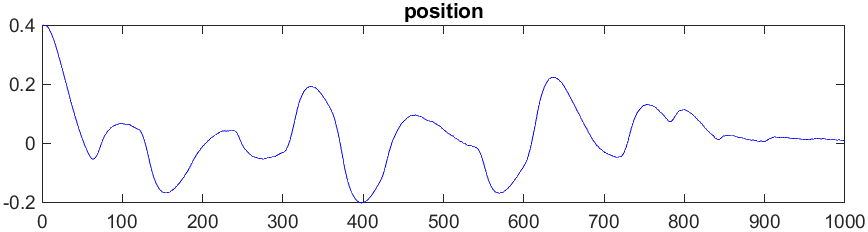
\includegraphics[width=150mm]{obr/posSmc.png}
	\caption{Position of the pendulum $($SMC simulation$)$.}\label{posSmc}
\end{figure}

\begin{figure}[!tbh]
	\centering
	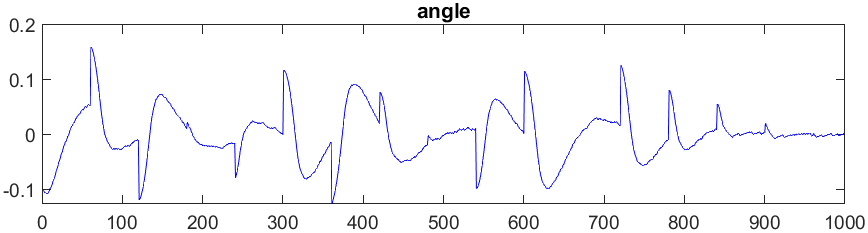
\includegraphics[width=150mm]{obr/angSmc.png}
	\caption{Angle of the pendulum $($SMC simulation$)$.}\label{angSmc}
\end{figure}

\begin{figure}[!tbh]
	\centering
	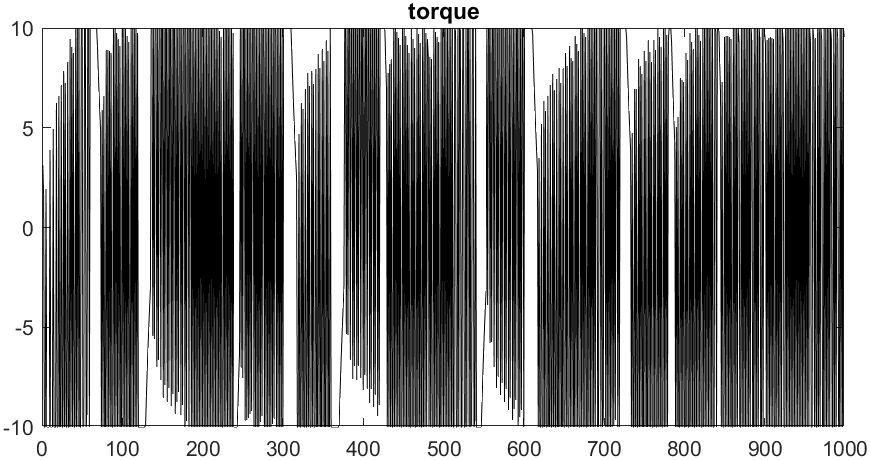
\includegraphics[width=150mm]{obr/torSmc.png}
	\caption{Torque of the pendulum $($SMC simulation$)$.}\label{torSmc}
\end{figure}

Examining the plots, it becomes apparent that the angle of the pendulum Fig. \ref{angSmc} achieves stabilization in the unstable upright position within a maximum of 40 samples, depending on the level of disturbance introduced. The position of the pendulum Fig. \ref{posSmc} attain stability within a maximum of 40 samples. We can clearly see the rapid switching of the control law on the Fig. \ref{torSmc}. 

\subsection{Implementation}

\newpage
\section{Fuzzy controller}
\subsection{Theory}
\subsection{Simulation}
\subsection{Implementation}

\newpage
\section{Impedance control}
\subsection{Theory}
\subsection{Simulation}
\subsection{Implementation}
	%\include{AeroShield}
	%\include{Software}
	%\include{Didakticke}
	%\include{matlabAsim}
	
	%%%%%%% end %%%%%%%%
	
	\bibliographystyle{unsrt}
	\pagenumbering{roman}\setcounter{page}{3}
	\addcontentsline{toc}{chapter}{Bibliography}
	\bibliography{bibliog}
	\backmatter
	\addcontentsline{toc}{section}{Source code of linear quadratic regulator (simulation)}
	\normalsize\bf{Source code of linear quadratic regulator (Simulation)}
\label{lqrSim.m}
\vspace{1cm}
\begin{lstlisting}[numbers=left,basicstyle=\scriptsize,caption={Source code of linear quadratic regulator (Simulation).},captionpos=b]	
clear all;
clc

%% Parameters and Initialization
Ts = 0.02; % Sampling Time
time = 20; % Total simulation time

% Preallocate arrays for system variables
q   = zeros(2, time/Ts); % Position and angle
qd  = zeros(2, time/Ts); % Linear and angular velocity
qdd = zeros(2, time/Ts); % Linear and angular acceleration
q(:, 1) = [0.4; -0.1]; % Initial values for position and angle
tau   = zeros(1, time/Ts); % Voltage
q_r(1) = 0;  % Reference value of position
q_r(2) = 0;  % Reference value of angle

qd_r = zeros(2, 1); % Reference value of linear and angular velocity

%% State-space
m_p     = 0.329; m_w     = 3.2; l_sp    = 0.44; f_w     = 6.2; 
f_p     = 0.009; gra       = 9.81; j_a     = 0.072; Ts = 0.02; 

% Continuous-time state-space matrices
A_c = [0   1                               0                   0
0   -f_w/(m_w+m_p)                  0                   0
0   0                               0                   1
0   (f_w*m_p*l_sp)/(j_a*(m_w+m_p)) (m_p*l_sp*gra)/j_a     -f_p/j_a];   
B_c = [0  ;   1/(m_w+m_p) ;   0   ;   -m_p*l_sp/((m_w+m_p)*j_a)];
C_c = [1   0   0   0
0   1   0   0
0   0   1   0
0   0   0   1];
D_c = [0;0;0;0];

% Convert to discrete-time
sys_cont = ss(A_c, B_c, C_c, D_c);
sys_d = c2d(sys_cont, Ts);

A = sys_d.A; B = sys_d.B; C = sys_d.C; D = sys_d.D;

%% Pendulum parameters
KF=2.6; M0=3.2; M1=0.329; M=M0+M1; ls=0.44; inert=0.072; N_val=0.1446;
N01_sq=0.23315; Fr=6.2; C=0.009; gra=9.81;

a32 = -N_val^2/N01_sq*gra ; a33 = -inert*Fr/N01_sq; a34 = N_val*C/N01_sq; 
a35 = inert*N_val/N01_sq; a42 = M*N_val*gra/N01_sq; a43 = N_val*Fr/N01_sq; a44 = -M*C/N01_sq;
a45 = -N_val^2/N01_sq; b3=inert/N01_sq; b4=-N_val/N01_sq;
b3_hat = inert/N01_sq+0.1; b4_hat = -N_val/N01_sq+0.1;

%% Animation parameters
xmin = -1;
xmax = +1;

figure;
h    = [];
h(1) = subplot(4,2,1);
h(2) = subplot(4,2,3);
h(3) = subplot(4,2,5);
h(4) = subplot(4,2,7);
h(5) = subplot(2,2,2);
h(6) = subplot(2,2,4);

Disturbance=1;

%% Controller Parameters
Q = diag([1, 1, 1e7, 1e2]);     % State penalization 
R = 1e7;                        % Input penalization
Np = 10;                        % Prediction horizon 
[K, P] = dlqr(A, B, Q, R);

for k = 1:time/Ts-1

% Control Algorithm
tau(1,k) = -K*[q(1,k); qd(1,k);q(2,k); qd(2,k)]; % LQR

% Voltage Limitation
if abs(tau(:,k)) > 10
tau(:,k) = sign(tau(:,k))*10;
end

% Inverted Pendulum Math. Model 
beta_x2 = (1 + N_val^2/N01_sq*(sin(q(2,k)))^2)^(-1);
qdd(:,k+1) = [beta_x2*(a32*sin(q(2,k))*cos(q(2,k))+a33*qd(1,k)+...
a34*cos(q(2,k))*(qd(2,k))+a35*sin(q(2,k))*qd(2,k)^2+b3*tau(:,k));
beta_x2*(a42*sin(q(2,k))+a43*cos(q(2,k))*qd(1,k)+...
a44*(qd(2,k))+a45*cos(q(2,k))*sin(q(2,k))*(qd(2,k))^2+b4*cos(q(2,k))*tau(:,k))];

qd(:,k+1) = qd(:,k) + qdd(:,k+1)*Ts;        
q(:,k+1) = q(:,k) + qd(:,k+1)*Ts;
q(2,k+1) = mod(q(2,k+1)+pi,2*pi)-pi;

% Disturbance
if mod(k,60)==0 && Disturbance==1
x = rand();

if x > 0.5 && k ~= 200
q(2,k+1) = q(2,k+1) + rand() * 0.12; 
else
q(2,k+1) = q(2,k+1) - rand() * 0.12; 
end

if k == 200
q(2,k+1) = q(2,k+1) - 0.1;  
end
end

% Plot Animation
plot(0, 'Parent', h(6));
hold on;
p1 = -q(1,k);
p2 = -q(1,k) + ls * exp(1i*(q(2,k)+pi/2));
line(real([p1,p2]), imag([p1,p2]));
plot(real(p2), imag(p2), '.', 'markersize', 40);
hold off;

% Center plot w.r.t. object
if q(1) > xmax
xmin = xmin + 0.1;
xmax = xmax + 0.1;
elseif q(1) < xmin
xmin = xmin - 0.1;
xmax = xmax - 0.1;
end

% Update animation
grid on;
axis([h(1)],[0 time/Ts-1 -1 1]); title('position')
axis([h(2)],[0 time/Ts-1 -0.5 0.5]); 
axis([h(3)],[0 time/Ts-1 -1 1]); 
axis([h(4)],[0 time/Ts-1 -5 5]); 
axis([h(5)],[0 time/Ts-1 -10 10]); 
axis([h(6)],[xmin-.2 xmax+.2 -.5 .5]);

% Update subplots
drawnow;

plot(q(1,1:k),'b','Parent',h(1)); %Position 
plot(q(2,1:k),'b','Parent',h(2)); % Angle 
plot(qd(1,1:k),'b','Parent',h(3)); % Velocity
plot(qdd(1,1:k),'b','Parent',h(4)); % Angular velocity
plot(tau(1:k),'k','Parent',h(5)); % Torque

title(h(1), 'Position');
title(h(2), 'Angle');
title(h(3), 'Velocity');
title(h(4), 'Angular Velocity');
title(h(5), 'Torque');
end
\end{lstlisting}
	\addcontentsline{toc}{section}{Source code of linear quadratic regulator (Real implementation)}
	\normalsize\bf{Source code of linear quadratic regulator (Real implementation)}
\label{lqrReal.m}
\vspace{1cm}
\begin{lstlisting}[numbers=left,basicstyle=\scriptsize,caption={Source code of linear quadratic regulator (Real implementation).},captionpos=b]	
% Pause for 3 seconds before starting the code execution
pause(3);

% Clear workspace, close all figures, and clear command window
clear all;
close all;
clc;

% Add necessary paths for libraries
addpath(genpath('CLSS Praxis'), genpath('hudaqlib'))

% Hudaq device initialization
dev = HudaqDevice('MF634');

% Total experiment samples
s = 2000;
% Sampling period
Ts = 0.02;

% States during the experiment
x = zeros(s,4);
% Sample states
z2 = zeros(4,1);
% Initial values
x(1,:) = [(AIRead(dev,1)/0.15/100) 0.01*round(-13.1*AIRead(dev,3)) (-AIRead(dev,2)/0.96*pi/180) 0];

% Force array to store calculated force values
Force = zeros(s,1);

% Pendulum parameters
m_p     = 0.329; m_w     = 3.2; l_sp    = 0.44; f_w     = 6.2; 
f_p     = 0.009; gra       = 9.81; j_a     = 0.072; Ts = 0.02; 

% Continuous-time state-space matrices
A_c = [ 0   1                               0                   0
0   -f_w/(m_w+m_p)                  0                   0
0   0                               0                   1
0   (f_w*m_p*l_sp)/(j_a*(m_w+m_p)) (m_p*l_sp*gra)/j_a     -f_p/j_a];   
B_c = [0  ;   1/(m_w+m_p) ;   0   ;   -m_p*l_sp/((m_w+m_p)*j_a)];
C_c = [   1   0   0   0
0   1   0   0
0   0   1   0
0   0   0   1];
D_c = [0;0;0;0];

% Convert to discrete-time
sys_cont = ss(A_c,B_c,C_c,D_c);
sys_d = c2d(sys_cont,Ts);

A = sys_d.A; B = sys_d.B; C = sys_d.C; D = sys_d.D;

% LQR controller parameters
Q = diag([100, .1, 100, .1]);    % State penalization 
R = 1e-2;                        % Input penalization
Np = 60;                         % Prediction horizon 
[K, P] = dlqr(A, B, Q, R);

% Loop through each sample
for i = 1:s-1

% LQR CONTROL ALGORITHM
Force(i) = ctranspose(-K*x(i,:));

% Save the data
z2(1) = AIRead(dev,1)/0.15/100;     % Position of cart (meter)
z2(2) = 0.01*round(-13.1*AIRead(dev,3));    % Speed of cart (m/s)
z2(3) = -AIRead(dev,2)/0.96*pi/180;  % Angle of pendulum (radian)

% Voltage limitation
if abs(Force(i)) > 10
Force(i) = sign(Force(i))*10; 
end

% Apply calculated voltage    
tic
while toc < Ts
DOWriteBit(dev, 1, 2, 1);   % Activation pendulum
DOWriteBit(dev, 1, 2, 0);   % Channel 1 consists of DO0..DO7
DOWriteBit(dev, 1, 2, 1);   % DO2 Requires continuous pulse
AOWrite(dev, 2, Force(i));  % Apply calculated voltage
end

% Angular speed calculation (derivative) 
z2_winkel = -AIRead(dev,2)/0.96*pi/180;
z2(4) = (z2_winkel - z2(3))/Ts;   % Angular speed of pendulum

% Update states
x(i+1,:) = ctranspose(z2);

% Check if the pendulum is out of range
if abs(z2(1)) > 0.3 || abs(z2(3)*180/pi) > 10    
disp('Please bring me back !');
pause(3);   % Wait for 3 seconds
end
\end{lstlisting}
	\addcontentsline{toc}{section}{Source code of model predictive controller (simulation)}
	\normalsize\bf{Source code of model predictive controller (Simulation)}
\label{mpcSim.m}
\vspace{1cm}
\begin{lstlisting}[numbers=left,basicstyle=\scriptsize,caption={Source code of model predictive controller (Simulation).},captionpos=b]	
% Clear workspace, command window, and import CasADi library
clear all;
clc

%% Parameters and Initialization
Ts = 0.02; % Sampling Time
time = 20; % Total simulation time

% Preallocate arrays for system variables
q   = zeros(2, time/Ts); % Position and angle
qd  = zeros(2, time/Ts); % Linear and angular velocity
qdd = zeros(2, time/Ts); % Linear and angular acceleration
q(:, 1) = [0.4; -0.1]; % Initial values for position and angle
tau   = zeros(1, time/Ts); % Voltage

q_r(1) = 0;  % Reference value of position
q_r(2) = 0;  % Reference value of angle
Q = diag([1, 1, 1e7, 1e2]);     % State penalisation 
R = 1e7;                        % Input penalisation
Np = 10;     % Prediction horizon 

qd_r = zeros(2, 1); % Reference value of linear and angular velocity

%% State-space
m_p     = 0.329; m_w     = 3.2; l_sp    = 0.44; f_w     = 6.2; 
f_p     = 0.009; gra       = 9.81; j_a     = 0.072; Ts = 0.02; 

% Continuous-time state-space matrices
A_c = [0   1                               0                   0
0   -f_w/(m_w+m_p)                  0                   0
0   0                               0                   1
0   (f_w*m_p*l_sp)/(j_a*(m_w+m_p)) (m_p*l_sp*gra)/j_a     -f_p/j_a];   
B_c = [0  ;   1/(m_w+m_p) ;   0   ;   -m_p*l_sp/((m_w+m_p)*j_a)];
C_c = [   1   0   0   0
0   1   0   0
0   0   1   0
0   0   0   1];
D_c = [0;0;0;0];

% Convert to discrete-time
sys_cont = ss(A_c,B_c,C_c,D_c);
sys_d = c2d(sys_cont,Ts);

A = sys_d.A; B = sys_d.B; C = sys_d.C; D = sys_d.D;
[K, P] = dlqr(A, B, Q, R);	% Linear quadratic regulator for callculating the P matrix

%% Pendulum parameters
KF=2.6; M0=3.2; M1=0.329; M=M0+M1; ls=0.44; inert=0.072; N_val=0.1446;
N01_sq=0.23315; Fr=6.2; C=0.009; gra=9.81;

a32 = -N_val^2/N01_sq*gra ; a33 = -inert*Fr/N01_sq; a34 = N_val*C/N01_sq; 
a35 = inert*N_val/N01_sq; a42 = M*N_val*gra/N01_sq; a43 = N_val*Fr/N01_sq; a44 = -M*C/N01_sq;
a45 = -N_val^2/N01_sq; b3=inert/N01_sq; b4=-N_val/N01_sq;
b3_hat = inert/N01_sq+0.1; b4_hat = -N_val/N01_sq+0.1;

%% Animation parameters
xmin = -1;
xmax = +1;

figure;
h    = [];
h(1) = subplot(4,2,1);
h(2) = subplot(4,2,3);
h(3) = subplot(4,2,5);
h(4) = subplot(4,2,7);
h(5) = subplot(2,2,2);
h(6) = subplot(2,2,4);

Disturbance = 1;

% Hessian, F matrices of cost function
[H, F] = Controller_MPC_CostFunction(A, B, Np, Q, R, P);
s = zeros(1, Np);
s(1, 1) = 1;

for k = 1:time/Ts-1

% CONTROL ALGORITHM - Explicit MPC
tau(1, k) = -s*(H^(-1))*F*[q(1, k); qd(1, k); q(2, k); qd(2, k)];

% Voltage limitation
if abs(tau(:, k)) > 10
tau(:, k) = sign(tau(:, k)) * 10;
end

% Inverted pendulum math model
beta_x2 = (1 + N_val^2/N01_sq*(sin(q(2, k)))^2)^(-1);
qdd(:, k+1) = [beta_x2*(a32*sin(q(2, k))*cos(q(2, k))+a33*qd(1, k)+...
a34*cos(q(2, k))*(qd(2, k))+a35*sin(q(2, k))*qd(2, k)^2+b3*tau(:, k));
beta_x2*(a42*sin(q(2, k))+a43*cos(q(2, k))*qd(1, k)+...
a44*(qd(2, k))+a45*cos(q(2, k))*sin(q(2, k))*(qd(2, k))^2+b4*cos(q(2, k))*tau(:, k))];

qd(:, k+1) = qd(:, k) + qdd(:, k+1)*Ts;        
q(:, k+1) = q(:, k) + qd(:, k+1)*Ts;
q(2, k+1) = mod(q(2, k+1) + pi, 2*pi) - pi;

% Disturbance
if mod(k, 60) == 0 && Disturbance == 1
x = rand();
if x > 0.5 && k ~= 200
q(2, k+1) = q(2, k+1) + rand()*0.12; 
else
q(2, k+1) = q(2, k+1) - rand()*0.12; 
end
if k == 200
q(2, k+1) = q(2, k+1) - 0.1;  
end
end

% Plotting animation
plot(0, 'Parent', h(6));
hold on;
p1 = -q(1, k);
p2 = -q(1, k) + ls*exp(1i*(q(2, k)+pi/2));
line(real([p1, p2]), imag([p1, p2]));
plot(real(p2), imag(p2), '.', 'markersize', 40);
hold off;

% Center plot w.r.t. object
if q(1) > xmax
xmin = xmin + 0.1;
xmax = xmax + 0.1;
elseif q(1) < xmin
xmin = xmin - 0.1;
xmax = xmax - 0.1;
end

grid on;
axis([h(1)], [0 time/Ts-1 -1 1]); title('position')
axis([h(2)], [0 time/Ts-1 -0.5 0.5]); 
axis([h(3)], [0 time/Ts-1 -1 1]); 
axis([h(4)], [0 time/Ts-1 -5 5]); 
axis([h(5)], [0 time/Ts-1 -10 10]); 
axis([h(6)], [xmin-.2 xmax+.2 -.5 .5]);

% Update animation
drawnow;

% Plotting system variables
plot(q(1, 1:k), 'b', 'Parent', h(1)); % Position 
plot(q(2, 1:k), 'b', 'Parent', h(2)); % Angle 
plot (qd(1, 1:k), 'b', 'Parent', h(3)); % Velocity
plot(qdd(1, 1:k), 'b', 'Parent', h(4)); % Angular velocity
plot(tau(1:k), 'k', 'Parent', h(5)); % Torque

title(h(1), 'position');
title(h(2), 'angle');
title(h(3), 'velocity');
title(h(4), 'angular velocity');
title(h(5), 'torque');
end
\end{lstlisting}
	\addcontentsline{toc}{section}{Source code of model predictive controller (Real implementation)}
	\normalsize\bf{Source code of model predictive controller (Real implementation)}
\label{mpcReal.m}
\vspace{1cm}
\begin{lstlisting}[numbers=left,basicstyle=\scriptsize,caption={Source code of model predictive controller (Real implementation).},captionpos=b]	
	% Pause for 3 seconds to allow initialization
	pause(3);
	
	% Clear workspace, close all figures, and clear command window
	clear all;
	close all;
	clc;
	
	% Add necessary paths for CLSS Praxis and hudaqlib
	addpath(genpath('CLSS Praxis'), genpath('hudaqlib'))
	
	% Create a HudaqDevice object for MF634
	dev = HudaqDevice('MF634');
	
	% Number of samples and sampling period
	s = 2000;    % Total experiment samples
	Ts = 0.02;   % Sampling period
	
	% Initialize arrays for storing system states and control input
	x = zeros(s, 4);     % States during the experiment
	z2 = zeros(4, 1);    % Sample states
	x(1, :) = [(AIRead(dev, 1)/0.15/100) 0.01*round(-13.1*AIRead(dev, 3)) (-AIRead(dev, 2)/0.96*pi/180) 0]; % Initial values
	Force = zeros(s, 1);  % Control input (force applied)
	
	%% State-space
	m_p = 0.329; m_w = 3.2; l_sp = 0.44; f_w = 6.2; 
	f_p = 0.009; gra = 9.81; j_a = 0.072; Ts = 0.02; 
	
	% Define continuous-time state-space matrices
	A_c = [ 0   1                               0                   0
	0   -f_w/(m_w+m_p)                  0                   0
	0   0                               0                   1
	0   (f_w*m_p*l_sp)/(j_a*(m_w+m_p)) (m_p*l_sp*gra)/j_a     -f_p/j_a];   
	B_c = [0  ;   1/(m_w+m_p) ;   0   ;   -m_p*l_sp/((m_w+m_p)*j_a)];
	C_c = [   1   0   0   0
	0   1   0   0
	0   0   1   0
	0   0   0   1];
	D_c = [0; 0; 0; 0];
	
	% Convert to discrete-time
	sys_cont = ss(A_c, B_c, C_c, D_c);
	sys_d = c2d(sys_cont, Ts);
	
	A = sys_d.A; B = sys_d.B; C = sys_d.C; D = sys_d.D;
	
	% Hessian, F matrices of cost function
	[H, F] = Controller_MPC_CostFunction(A, B, Np, Q, R, P);
	a = zeros(1, Np);
	a(1, 1) = 1;
	
	for i = 1:s-1

	% MPC CONTROL ALGORITHM
	Force(i) = ctranspose(-a*(H^(-1))*F*x(i, :));
	
	% Save the data
	z2(1) = AIRead(dev, 1)/0.15/100;         % Position of the cart (meter)
	z2(2) = 0.01*round(-13.1*AIRead(dev, 3)); % Speed of the cart (m/s)
	z2(3) = -AIRead(dev, 2)/0.96*pi/180;      % Angle of the pendulum (radian)
	
	% Voltage limitation
	if abs(Force(i)) > 10
	Force(i) = sign(Force(i))*10; 
	end
	
	% Apply calculated voltage    
	tic
	while toc < Ts
	DOWriteBit(dev, 1, 2, 1);  % Freischaltung Pendel
	DOWriteBit(dev, 1, 2, 0);  % Channel 1 consists of DO0..DO7
	DOWriteBit(dev, 1, 2, 1);  % DO2 Requires continuous pulse
	AOWrite(dev, 2, Force(i)); % Apply calculated voltage
	end
	
	% Angular speed calculation (derivative) 
	z2_winkel = -AIRead(dev, 2)/0.96*pi/180;
	z2(4) = (z2_winkel - z2(3))/Ts; % Angular speed of the pendulum
	
	% Update system states
	x(i+1, :) = ctranspose(z2);
	
	% Check if the pendulum is out of range
	if abs(z2(1)) > 0.3 || abs(z2(3)*180/pi) > 10    % Der Pendel ist ausser Bereich
	disp('Please bring me back !');
	pause(3);  % Wait 3 seconds
	end
\end{lstlisting}
	\addcontentsline{toc}{section}{Source code of cost function callculation for MPC}
	\normalsize\bf{Source code of cost function callculation for MPC}
\label{mpcCostFcn.m}
\vspace{1cm}
\begin{lstlisting}[numbers=left,basicstyle=\scriptsize,caption={Source code of cost function callculation for MPC.},captionpos=b]	
function [H, F] = CostFunctionMPC(A, B, np, Q, R, P)

[nx, nu] = size(B);         % Get system dimensions

phi = zeros(np*nx, nx);       % Preallocate matrix Phi
for i = 1:np                  % Create matrix M using powers of matrix A
phi(i*nx-nx+1:i*nx, :) = A^i; 
end

% Get prediction matrix N
gamma = zeros(nx*np, nu*np);    % Preallocate matrix Gamma
NN = zeros(nx*np, nu);          % Preallocate auxiliary matrix NN with zeros
for i = 1:np                    % Calculate auxiliary matrix NN
NN(i*nx-nx+1:i*nx, :) = A^(i - 1) * B; 
end
for i = 1:np                % By shifting NN matrix create matrix Gamma
gamma(i*nx-nx+1:end, i*nu-nu+1:i*nu) = NN(1:np*nx-(i - 1)*nx, :); 
end

% Get cost function matrices H,F
psi = kron(eye(np), R);
omega = zeros(np*nx, np*nx);  % Preallocate matrix Omega
for i = 1:np-1                % Create matrix Omega
omega(i*nx-nx+1:i*nx, i*nx-nx+1:i*nx) = Q; 
end
omega(np*nx-nx+1:np*nx, np*nx-nx+1:np*nx) = P; % Add last diagonal element
H=2*(psi+gamma'*omega*gamma);
F=2*gamma'*omega*phi;

end
\end{lstlisting}
	\addcontentsline{toc}{section}{Source code of sliding mode controller (simulation)}
	\normalsize\bf{Source code of sliding mode controller (Simulation)}
\label{smcSim}
\vspace{1cm}
\begin{lstlisting}[numbers=left,basicstyle=\scriptsize,caption={Source code of sliding mode controller (Simulation).},captionpos=b]	
clear all;
clc;

%% Parameters and Initialization
Ts = 0.02; % Sampling Time
time = 20; % Total simulation time
alpha = 6;
beta = 1.8; % Variable that changes the speed of switching or duty cycle
var_k = 10;

% Initial values
q = zeros(2, time / Ts); % Position and angle
qd = zeros(2, time / Ts); % Linear and angular velocity
qdd = zeros(2, time / Ts); % Linear and angular acceleration
q(:, 1) = [0.4; -0.1]; % Initial values for position and angle
tau = zeros(1, time / Ts); % Voltage

q_r(1) = 0; % Reference value of position
q_r(2) = 0; % Reference value of angle

qd_r = zeros(2, 1); % Reference value of linear and angular velocity

%% State-space
% Define system matrices for continuous-time and discrete-time systems
m_p = 0.329; m_w = 3.2; l_sp = 0.44; f_w = 6.2;
f_p = 0.009; gra = 9.81; j_a = 0.072; Ts = 0.02;

A_c = [0 1 0 0;
0 -f_w / (m_w + m_p) 0 0;
0 0 0 1;
0 (f_w * m_p * l_sp) / (j_a * (m_w + m_p)) (m_p * l_sp * gra) / j_a -f_p / j_a];
B_c = [0; 1 / (m_w + m_p); 0; -m_p * l_sp / ((m_w + m_p) * j_a)];
C_c = [1 0 0 0;
0 1 0 0;
0 0 1 0;
0 0 0 1];
D_c = [0; 0; 0; 0];

% Convert to discrete-time system
sys_cont = ss(A_c, B_c, C_c, D_c);
sys_d = c2d(sys_cont, Ts);

A = sys_d.A; B = sys_d.B; C = sys_d.C; D = sys_d.D;

%% Pendulum parameters
KF = 2.6; M0 = 3.2; M1 = 0.329; M = M0 + M1; ls = 0.44; inert = 0.072; N_val = 0.1446;
N01_sq = 0.23315; Fr = 6.2; C = 0.009; gra = 9.81;

% Define coefficients for inverted pendulum math model
a32 = -N_val^2 / N01_sq * gra; a33 = -inert * Fr / N01_sq; a34 = N_val * C / N01_sq;
a35 = inert * N_val / N01_sq; a42 = M * N_val * gra / N01_sq; a43 = N_val * Fr / N01_sq;
a44 = -M * C / N01_sq; a45 = -N_val^2 / N01_sq; b3 = inert / N01_sq; b4 = -N_val / N01_sq;
b3_hat = inert / N01_sq + 0.1; b4_hat = -N_val / N01_sq + 0.1;

%% Animation parameters
xmin = -1;
xmax = +1;

% Create subplots for animation
figure;
h = [];
h(1) = subplot(4, 2, 1);
h(2) = subplot(4, 2, 3);
h(3) = subplot(4, 2, 5);
h(4) = subplot(4, 2, 7);
h(5) = subplot(2, 2, 2);
h(6) = subplot(2, 2, 4);

Disturbance = 1;

%% Control
for k = 1:time / Ts - 1
% Control algorithm
s = -qd(2, k) - alpha * q(2, k) - qd(1, k) - beta * q(1, k);
tau(1, k) = 12.335239 * qd(1, k) + 68.877358 * q(2, k) - 3.492138 * (0.125 - alpha) * qd(2, k)...
- 3.492138 * (1.7568 - beta) * qd(1, k) - (var_k * sign(s));

% Voltage limitation
if abs(tau(:, k)) > 10
tau(:, k) = sign(tau(:, k)) * 10;
end

% Inverted pendulum math model
beta_x2 = (1 + N_val^2 / N01_sq * (sin(q(2, k)))^2)^(-1);
qdd(:, k + 1) = [beta_x2 * (a32 * sin(q(2, k)) * cos(q(2, k)) + a33 * qd(1, k) + ...
a34 * cos(q(2, k)) * (qd(2, k)) + a35 * sin(q(2, k)) * qd(2, k)^2 + b3 * tau(:, k));
beta_x2 * (a42 * sin(q(2, k)) + a43 * cos(q(2, k)) * qd(1, k) + ...
a44 * (qd(2, k)) + a45 * cos(q(2, k)) * sin(q(2, k)) * (qd(2, k))^2 + b4 * cos(q(2, k)) * tau(:, k))];

% Update position and velocity
qd(:, k + 1) = qd(:, k) + qdd(:, k + 1) * Ts;
q(:, k + 1) = q(:, k) + qd(:, k + 1) * Ts;
q(2, k + 1) = mod(q(2, k + 1) + pi, 2 * pi) - pi;

% Disturbance
if mod(k, 60) == 0 && Disturbance == 1
x = rand();

if x > 0.5 && k ~= 200
q(2, k + 1) = q(2, k + 1) + rand() * 0.12;
else
q(2, k + 1) = q(2, k + 1) - rand() * 0.12;
end

if k == 200
q(2, k + 1) = q(2, k + 1) - 0.1;
end
end

% Animation
plot(0, 'Parent', h(6));
hold on;
p1 = -q(1, k);
p2 = -q(1, k) + ls * exp(1i * (q(2, k) + pi / 2));
line(real([p1, p2]), imag([p1, p2]));
plot(real(p2), imag(p2), '.', 'markersize', 40);
hold off;

% Center plot w.r.t. object
if q(1) > xmax
xmin = xmin + 0.1;
xmax = xmax + 0.1;
elseif q(1) < xmin
xmin = xmin - 0.1;
xmax = xmax - 0.1;
end
grid on;
axis([h(1)], [0 time / Ts - 1 -1 1]);
title('position');
axis([h(2)], [0 time / Ts - 1 -0.5 0.5]);
title('angle');
axis([h(3)], [0 time / Ts - 1 -1 1]);
title('velocity');
axis([h(4)], [0 time / Ts - 1 -5 5]);
title('angular velocity');
axis([h(5)], [0 time / Ts - 1 -10 10]);
title('torque');

% Update animation
drawnow;

% Plot results
plot(q(1, 1:k), 'b', 'Parent', h(1)); % Position
plot(q(2, 1:k), 'b', 'Parent', h(2)); % Angle
plot(qd(1, 1:k), 'b', 'Parent', h(3)); % Velocity
plot(qdd(1, 1:k), 'b', 'Parent', h(4)); % Angular velocity
plot(tau(1:k), 'k', 'Parent', h(5)); % Torque
title(h(1), 'position');
title(h(2), 'angle');
title(h(3), 'velocity');
title(h(4), 'angular velocity');
title(h(5), 'torque');
end
\end{lstlisting}
	\addcontentsline{toc}{section}{Source code of sliding mode controller (Real implementation)}
	\normalsize\bf{Source code of sliding mode controller (Real implementation)}
\label{smcReal}
\vspace{1cm}
\begin{lstlisting}[numbers=left,basicstyle=\scriptsize,caption={Source code of sliding mode controller (Real implementation).},captionpos=b]	
pause(3);
clear all;
close all;
clc;

addpath(genpath('CLSS Praxis'),genpath('hudaqlib'))
dev = HudaqDevice('MF634');
mn = 25;
mkdir Messung_25;

s = 2000;  %total experiment sample
Ts = 0.02; % sampling period

x = zeros(s,4); %states during experiment
z2 = zeros(4,1);% sample states
x(1,:) = [(AIRead(dev,1)/0.15/100) 0.01*round(-13.1*AIRead(dev,3)) (-AIRead(dev,2)/0.96*pi/180) 0]; % inital values
Force = zeros(s,1); 

%% State-space
m_p     = 0.329;m_w     = 3.2;l_sp    = 0.44;f_w     = 6.2; 
f_p     = 0.009;gra       = 9.81;j_a     = 0.072;Ts = 0.02; 

A_c = [ 0   1                               0                   0
0   -f_w/(m_w+m_p)                  0                   0
0   0                               0                   1
0   (f_w*m_p*l_sp)/(j_a*(m_w+m_p)) (m_p*l_sp*gra)/j_a     -f_p/j_a];   
B_c = [0  ;   1/(m_w+m_p) ;   0   ;   -m_p*l_sp/((m_w+m_p)*j_a)];
C_c = [   1   0   0   0
0   1   0   0
0   0   1   0
0   0   0   1];
D_c = [0;0;0;0];

sys_cont = ss(A_c,B_c,C_c,D_c);
sys_d = c2d(sys_cont,Ts);

A = sys_d.A;B = sys_d.B;C = sys_d.C;D = sys_d.D;

%% Implementation
alpha = 6;  
beta = 1.8; % variable that changes the speed of switching resp the duty cycle
var_k = 10;

for i = 1:s-1

%  CONTROL ALGORITHM

s1 = - x(i,4) - alpha * x(i,3)- x(i,2)- beta * x(i,1); 
Force(i) = 12.335239*x(i,2)+68.877358*x(i,3)-3.492138*(0.125-alpha)*x(i,4)-3.492138*(1.7568-beta)*x(i,2)-(var_k * sign(s1));

% save the data
z2(1) = AIRead(dev,1)/0.15/100; % position of cart (meter)
z2(2) = 0.01*round(-13.1*AIRead(dev,3)); % speed of cart (m/s)
z2(3) = -AIRead(dev,2)/0.96*pi/180; % angle of pendulum (radian)

% voltage limitation
if abs(Force(i))>10
Force(i) = sign(Force(i))*10; 
end

% apply calculated voltage    
tic
while toc<Ts
DOWriteBit(dev,1,2,1)           % Freischaltung Pendel
DOWriteBit(dev,1,2,0)           % channel 1 besteht aus DO0..DO7
DOWriteBit(dev,1,2,1)           % DO2 requires continuous impuls
AOWrite(dev, 2, Force(i));      % apply calculated voltage
end

% angular speed calculation (derivative) 
z2_winkel = -AIRead(dev,2)/0.96*pi/180;
z2(4) = (z2_winkel-z2(3))/Ts; % angular speed of pendulum

x(i+1,:) = z2';

if abs(z2(1)) > 0.3 || abs(z2(3)*180/pi) > 10    % Der Pendel ist ausser Bereich
disp('Please bring me back !');
pause(3);                 % wait 3 second
end

end
\end{lstlisting}
\end{document}